\section{Benchmarking} \label{benchmarking}
We used datasets of 2 different sizes to perform the benchmarking of the
application. Table \ref{tab:datasets} shows the details of the two datasets.
The CreateWord2VecModel spark application is most complex and time
consuming application. We used this application for the benchmarking. We
deployed the application on Chameleon cloud and Jetstream cloud. Table
\ref{tab:cloudconfig} shows the details for the cluster configurations on
Chameleon and Jetstream clouds.

\begin{table}[htbp]
\centering
\caption{\bf Dataset Used for Performance Measurement}
  \begin{tabular}{l|c|r}
    \hline
    Parameter & Dataset1 & Dataset2 \\
    Size of crawldb & 1.4MB & 7.4MB \\
    Count of files in crawldb & 100 & 500 \\
    Source & Wikipedia & Wikipedia \\
    \hline
  \end{tabular}
  \label{tab:datasets}
\end{table}


\begin{table}[htbp]
\centering
\caption{\bf Dataset Used for Performance Measurement}
  \begin{tabular}{ l | c | r }
    \hline
    Parameter & Chameleon Cluster & Jetstream Cluster \\
    Cluster name & cluster-005 & cluster-010 \\
    Nodes & 2 & 2 \\
    OS & Ubuntu 14.04 & Ubuntu 14.04 \\
    Flavor & m1.medium & m1.medium \\
    Secgroup & default & default \\
    Assign floating IP & True & True \\
    Cloud & chameleon & iujetstream \\
    \hline
  \end{tabular}
  \label{tab:cloudconfig}
\end{table}


Figure \ref{fig:compare147} shows the total time taken by CreateWord2Vec
application for Dataset1 on the Chameleon and Jetstream cloud environments.
\begin{figure}[htbp]
\centering
\fbox{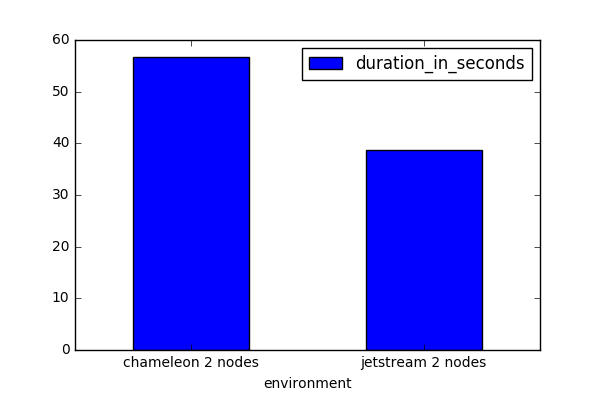
\includegraphics[width=\linewidth]{images/compare147.png}}
\caption{Time taken by CreateWord2Vec for Dataset1}
\label{fig:compare147}
\end{figure}

Figure \ref{fig:compare522} shows the total time taken by CreateWord2Vec
application for Dataset2 on the Chameleon and Jetstream cloud environmentnments.
\begin{figure}[htbp]
\centering
\fbox{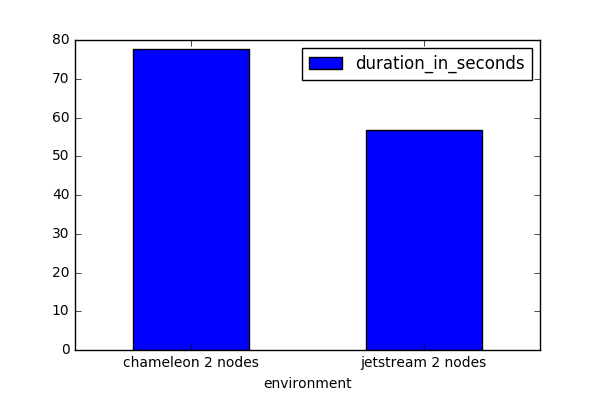
\includegraphics[width=\linewidth]{images/compare522.png}}
\caption{Time taken by CreateWord2Vec for Dataset2}
\label{fig:compare522}
\end{figure}

\subsection{Working with large dataset} \label{benchmarklargedatasets}
There are several configuration parameters added in the application to
fine tune the behavior of the spark applications. When working with larger
datasets, the spark applications can go out of memory. Following parameters
can be configured in the config.propertise to handle such situation.

\begin{verbatim}
spark_executor_memory = <memory given to executor>
spark_driver_memory = <memory given to driver>
max_result_size = <maximum result size>
\end{verbatim}

We tried running out solution on a 4 node cluster with 1000 files on
the crawlDB and the create model script failed with out
of memory exceptions.

\begin{verbatim}
["OpenJDK 64-Bit Server VM warning: 
INFO: os::commit_memory(0x00007ff67449f000, 12288, 0) 
failed; error='Cannot allocate memory' (errno=12)", 
"OpenJDK 64-Bit Server 
VM warning: INFO: 
os::commit_memory(0x00007ff6746a1000, 12288, 0) 
failed; error='Cannot allocate memory' (errno=12)", "#", "# 
There is insufficient memory for the Java Runtime 
Environment to continue.", 
"# Native memory allocation (malloc) failed to 
allocate 12288 bytes for committing reserved memory.", 
"# An error report file with more information is saved as:", 
"# /home/hadoop/hs_err_pid25854.log"], "warnings": []}
\end{verbatim}

We need to tune spark memory parameters here, since the words in model 
become too high and we need as much memory(RAM) to execute the
solution or else it goes out of memory(OOM). For example for 
min\_word\_count = 5, the number of words in the model were 20839 
and executor\_memory of 4GB was enough. But for min\_word\_count of 3 
which resulted in 30194 words in model, we have to give 6GB RAM. After
making these changes to spark executor and driver memory 
we were able to run the solution successfully with 1000 files. 

\begin{table}[htbp]
\centering
\caption{\bf Cluster configuration used for performance measurement}
  \begin{tabular}{ l | c }
    \hline
    Parameter & Chameleon Cluster  \\
    Cluster name & cluster-006 \\
    Nodes & 4  \\
    OS & Ubuntu 14.04  \\
    Flavor & m1.medium \\
    Secgroup & default  \\
    Assign floating IP & True  \\
    Cloud & chameleon \\
    \hline
  \end{tabular}
  \label{tab:cloud4node}
\end{table}

Figure \ref{fig:compare_mwc_5_3} shows the total time taken by CreateWord2Vec
application varying min word count on the Chameleon cloud using 
min\_word\_count 3 and 5.
\begin{figure}[htbp]
\centering
\fbox{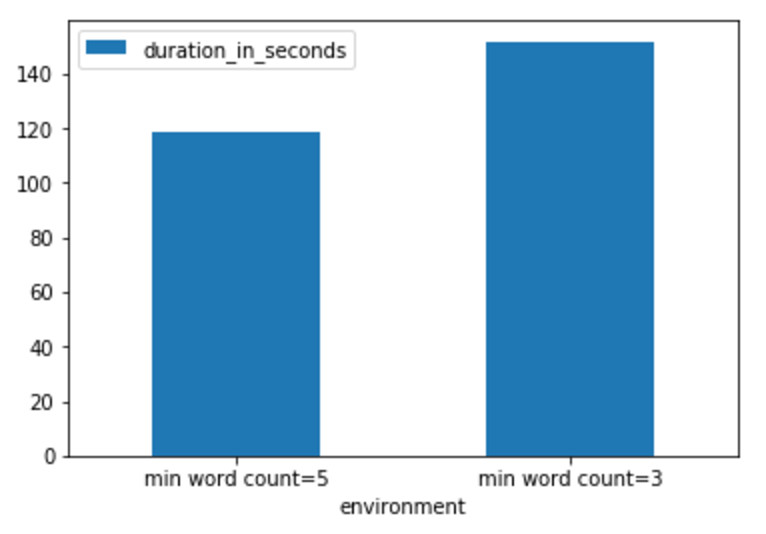
\includegraphics[width=\linewidth]{images/compare_mwc_5_3}}
\caption{Time taken when min word count varies from 3 to 5}
\label{fig:compare_mwc_5_3}
\end{figure}

Figure \ref{fig:compare_mwc_10_8} shows the total time taken by CreateWord2Vec
application varying min word count values from 8 to 10 on the Chameleon cloud using 
min\_word\_count 10 and 8.
\begin{figure}[htbp]
\centering
\fbox{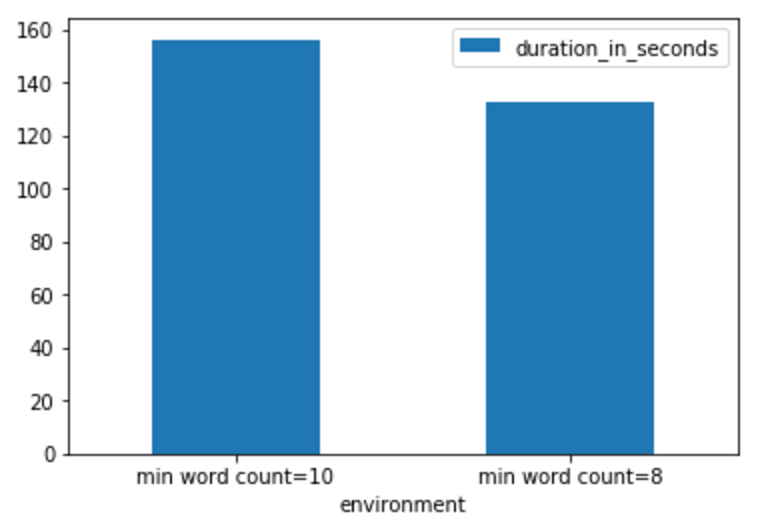
\includegraphics[width=\linewidth]{images/compare_mwc_10_8}}
\caption{Time taken when min word count varies from 8 to 10}
\label{fig:compare_mwc_10_8}
\end{figure}



